\chapter{Proposta para análise de arquiteturas \ac{mmorpg}}
\label{cap3}



As arquiteturas de serviços \ac{mmorpg} são desenvolvidas visando suprir as necessidades do \textit{design} do jogo desenvolvido, de forma a viabilizar a utilização deste serviço.
%
Nesse sentido, jogos com mecânicas de \textit{design} parecidos possuem implementações parecidas para os clientes.
%
Entretanto, a arquitetura escolhida impacta no custo de operação e qualidade do serviço aos jogadores.
%
Por este motivo, diferentes arquiteturas com o mesmo \textit{design} não são comparáveis entre sí, visto que dependem das regras de negócio do \textit{design} do jogo.



Ao desenvolver um serviço \ac{mmorpg} é necessário decidir uma arquitetura na qual reduza custos, consumo de recursos e minimize ocorrências para os jogadores a fim de viabilizar o seu comércio como produto.
%
Porém, a impossibilidade de comparação direta entre as arquiteturas de serviço \ac{mmorpg} instiga a análise das características básicas destas arquiteturas que possam influenciar o \textit{game design}, tais como consumo de recursos, tempo de resposta, latência e número máximo de clientes simultâneos conectados nos microsserviços.
%
Sendo assim, uma análise do consumo de recursos computacionais das arquiteturas levantadas previamente na literatura tem valor científico no auxílio na escolha de implementações arquiteturas de microsserviços, em específico para serviços \ac{mmorpg}.



Nesta seção é descrito a proposta para análise de consumo de recursos computacionais em arquiteturas \ac{mmorpg}.
%
A atual seção descreve a Proposta (Subseção~\ref{sec:proposta}), trazendo os objetivos desta análise, quais recursos e métricas serão analisadas.
%
Os Critérios de Análise (Subseção~\ref{sec:criterios}) exibem como os dados obtidos devem ser interpretados, baseando-se nos objetivos da análise das arquiteturas.
%
O Plano de Testes (Subseção~\ref{sec:plano}) exibe como será realizada a coleta dos dados, descrevendo cenários, critérios e objetivos dos testes.



\section{Proposta}
\label{sec:proposta}

Tendo analisado os trabalhos relacionados e as arquiteturas específicas para jogos \ac{mmorpg}, o presente trabalho tem como objetivo analisar as arquiteturas \ac{mmorpg} visando complementar a análise de arquitetura e consumo de recursos computacionais não analisados nos trabalhos relacionados.
%
Em específico, serão obtidos das arquiteturas Rudy (Subseção~\ref{rudy}), Salz (Subseção~\ref{salz}) e Willson (Subseção~\ref{willson}) os seguintes valores referentes aos recursos computacionais (Tabela~\ref{tab:recursos_categoria}):

\begin{enumerate}
  \item \textbf{\ac{cpu}}: o uso de CPU, com sua representação sendo em relação a porcentagem dos núcleos utilizados;
  \item \textbf{Memória}: Quantia de memória utilizada pelos processos da máquina. A sua representação será como dado absoluto;
  \item \textbf{Rede}: Serão obtidos os valores de entrada e saída de cada microsserviço, utilizando valores absolutos. Também será obtido o valor de latência do cliente ao microsserviço, para analisar o congestionamento da rede, a qual será representado em milissegundos.
\end{enumerate}

Além dos recursos computacionais, esta análise levará em conta valores referentes a outras métricas.
%
As métricas, cujos os valores serão obtidos são:

\begin{enumerate}
  \item \textbf{Número máximo de jogadores simultâneos}: Descobrir o limite de conexões para as arquiteturas propostas a análise. Será representado como valor absoluto.
  \item \textbf{Tempo de resposta das requisições}: Descobrir o tempo de resposta por categoria de requisição, conforme o número de jogadores no serviço. Será representado como tempo decorrido, em milissegundos.
\end{enumerate}

Todos estes valores serão obtidos a partir de simulações, e por este motivo se faz necessário descrever o comportamento dos jogadores simulados.
%
Espera-se em situações adversas, caracterizar os comportamentos das arquiteturas, gargalos e os custos de recursos computacionais para manutenção das arquiteturas de microsserviços.
%
Para este fim, se faz necessário a descrição dos critérios que serão utilizados durante a análise dos valores obtidos nos experimentos.

%ccm
% objetivos
% Definição das métricas para os itens levantados nas Tabelas 2.4 e 2.5

\section{Critérios de análise}
\label{sec:criterios}

A fim de padronizar a análise dos dados obtdos, a seção Critérios de Análise irá descrever como será guiada a análise conforme o coportamento dos valores obtidos.
%
Neste sentido, a análise dos dados obtidos serão guiadas pelo esperado dos valores obtidos em um serviço perfeito:

\begin{enumerate}
  \item \textbf{CPU}: Espera-se estressar com um elevado número de requisições.
  \item \textbf{Memória}: Espera-se estressar com requisições na qual exija armazenamento em memória.
  \item \textbf{Rede - Entrada}: Espera-se estressar com requisições na qual tenham uma carga de dados elevada.
  \item \textbf{Rede - Saída}: Espera-se estressar com respostas na qual tenham uma carga de dados elevada.
  \item \textbf{Número de Conexões}: Servirá como guia de comparação com os demais valores e desempenho da arquitetura;
  \item \textbf{Tempo de resposta das requisições}: Servira como guia de desempenho da arquitetura;
  \item \textbf{Latência}: Servirá como guia de comparação com os demais valores;
\end{enumerate}

Em um caso de uso perfeito, todos os recursos não são estressáveis, com um número de conexões simultâneas elevado.
%
Porém, espera-se para o atual trabalho um possível conjunto de ocorrências, na qual podem ou não ocorrer.
%
Este conjunto servirá de guia / exemplo de problemas relevantes retirado dos valores obtidos.
%
Logo, a simulação e cenários serão desenhados para forçar tais ocorrências.


A partir dos valores obtidos e seguindo o esperado de uma arquitetura totalmente relacionada ao número de conexões, espera-se encontrar um conjunto de eventuais problemas nas arquiteturas.
%
Um conjunto exemplo destes problemas são exibidos na Tabela~\ref{tab:problemas}.

\begin{table}[htb!]
  \centering
  \caption{Possíveis conjuntos para a anáise}
  \label{tab:problemas}
  \begin{tabular}{|l|l|l|l|l|l|l|l|}
  \hline
  \multicolumn{7}{|c|}{Recursos}                                                                      & \multirow{2}{*}{Descrição} \\ \cline{1-7}
  \rotatebox[origin=c]{90}{\ac{cpu}} & \rotatebox[origin=c]{90}{Memória} & \rotatebox[origin=c]{90}{Rede Entrada} & \rotatebox[origin=c]{90}{Rede Saída} & \rotatebox[origin=c]{90}{Conexões Simultâneas} & \rotatebox[origin=c]{90}{Tempo de Resposta} & \rotatebox[origin=c]{90}{Latência} &                            \\ \hline
  $\uparrow$    &              &              &              & $\downarrow$ &              &              & \thead{Rotina de processamento de requisições\\está ocupando muita \ac{cpu}} \\ \hline
                & $\uparrow$   &              &              & $\downarrow$ &              &              & \thead{O microsserviço está armazenando\\informações a qual poderiam estar em outros\\microsserviços}  \\ \hline
                &              & $\uparrow$   &              & $\downarrow$ &              &              & \thead{Uma entrada de dados elevada pode indicar\\o uso de um protocolo\\indapropriado para o serviço} \\ \hline
                &              &              & $\uparrow$   & $\downarrow$ &              &              & \thead{Caso a saída esteja muito elevada\\pode indicar uma má configuração de elementos\\que são transitados na rede ou\\uso inadequado de protocolos} \\ \hline
                &              &              &              & $\downarrow$ & $\uparrow$   &              & \thead{Pode estar relacionado\\a desempenho de processamento\\, modelo de paralelismo ou congestionamento de rede} \\ \hline
                &              &              &              & $\downarrow$ & $\uparrow$   & $\uparrow$   & \thead{Está relacionado com\\ congestionamento da rede} \\ \hline
  $\downarrow$  &              & $\uparrow$   & $\uparrow$   &              &              &              & \thead{Possível gargalo na rede\\ou protocolo ineficiente} \\ \hline
  $\uparrow$    & $\uparrow$   & $\downarrow$ & $\downarrow$ &              &              &              & \thead{Possível gargalo nos algoritmos\\utilizados no serviço} \\ \hline
                &              &              &              & $\downarrow$ &              &              & \thead{Bloqueio de novas conexões pelo\\sistema operacional ou\\modelo de paralelismo} \\ \hline
  $\uparrow$    & $\uparrow$   & $\uparrow$   & $\uparrow$   & $\uparrow$   & $\uparrow$   &  $\uparrow$  & \thead{Limite de processamento da arquitetura} \\ \hline
  $\downarrow$  & $\downarrow$ & $\downarrow$ & $\downarrow$ & $\uparrow$   & $\downarrow$ &  $\downarrow$& \thead{Teste perfeito} \\ \hline


  \end{tabular}

  Fonte: O próprio autor.
\end{table}

A Tabela~\ref{tab:problemas} relaciona os recursos conforme dois padrões:

\begin{itemize}
  \item Valores acima da média ($\uparrow$): Fazem referência a valores acima da média, comparado ao seu limite.
  \item Valores baixo da média ($\downarrow$): Fazem referência a valores acima da média, comparado ao seu limite.
\end{itemize}

Entretanto, espera-se encontrar problemas mais detalhados, além de problemas padronizados de forma genérica na Tabela~\ref{tab:problemas}.
%
Espera-se encontrar eventuais problemas conforme o tipo de requisição e desenho da arquitetura.
%
Estes problemas servirão para guiar a analise final das arquiteturas.

Seguindo estes critérios da análise, se faz necessário definir um plano de testes para obter os dados conforme os cenários e casos de uso do atual trabalho.

%ccm
% Identificar como os valores obtidos pelas métricas devem ser interpretados
% pode ser individdual ou em grupos, defiir a finalidade? Custo? Desempenho?

%ccm Usar os critérios das colunas das Tabelas 2.4 e 2.5 de modo a deixar clara a importância de realizar uma análise que contemple todos os itens e não apenas partes deles, como identificado nos trabalahos relacionados (Seção 2.7).

\section {Plano de testes}
\label{sec:plano}



O plano de testes definirá os cenários que serão aplicados sobre todas as arquiteturas de microsserviços para jogos \ac{mmorpg}.
%
Ele servirá para descrever formas de estressar as arquiteturas, a fim de obter os valores para análise.
%
Entretanto, antes de relatar os cenários de teste, se faz necessário descrever o ambiente onde ocorrerá tais testes.
%
A Figura~\ref{Ambiente de testes} descreve a infraestrutura utilizada para execução das camadas de aplicação utilizados nos testes.



\begin{figure}[htb!]
  \caption{Ambiente de testes definido para a coleta de dados}
  \label{Ambiente de testes}
  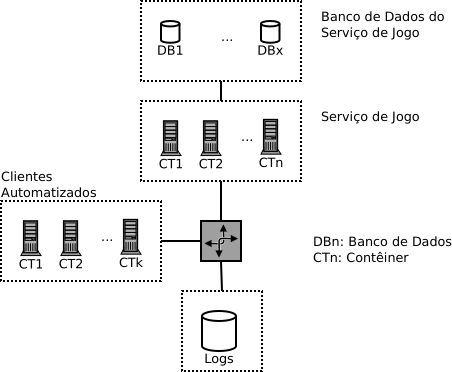
\includegraphics[height=6.5cm]{img/cap3/infraestrutura.png}
  \centering

  Fonte: O próprio autor.
\end{figure}



Como visível na Figura~\ref{Ambiente de testes}, o ambiente de testes planejado está segregado em 5 camadas.
%
Essas camadas tem o objetivo de diminuir o impacto de desempenho e consumo de recursos por outras ferramentas durante os testes.
%
Por este motivo, as regiões da infraestrutura planejada são:



\begin{enumerate}
  \item \textbf{Serviço de Jogo}: A camada de serviço da infraestrutura dos testes concentrará a arquitetura de microsserviços referente as arquiteturas de microsserviços analisadas.
  \item \textbf{Banco de dados do serviço de jogo}: A camada de banco de dados do serviço de jogo conterá os serviços de dados e web a fim de manter um padrão de banco de dados para ambos os serviços utilizados e auxiliar na inicialização dos testes.
  \item \textbf{Estresse}: A camada de estresse será responsável por realizar requisições ao serviço a fim de estressá-lo, simulando padrões de requisição de um padrão de um jogador.
  \item \textbf{Cliente}: A camada de cliente será composta pelos mesmos elementos da camada de estresse, porém em um ambiente controlado para que a suíte de estresse não interfira nas métricas obtidas no lado do cliente.
  \item \textbf{Dados}: A camada de dados será composta por algum banco de dados de log a fim de armazenar os dados obtidos da camada Cliente e serviço, para utilizar na análise.
\end{enumerate}



As regiões da infraestrutura utilizada no ambiente de testes deve manter um padrão a fim que não exista interferência entre os testes, além do desempenho das arquiteturas do serviço.
%
Espera-se utilizar em grande parte o mesmo sistema de cliente para ambas as arquiteturas, excluso casos onde a arquitetura necessite de alterações.
%
Nesse sentido, espera-se obter somente a interferência das arquiteturas expressa nos valores obtidos.



Para os casos de uso, serão utilizada as arquiteturas de microsserviços específicos a jogos \ac{mmorpg} obtidos da literatura.
%
São essas elas:



\begin{enumerate}
  \item \textbf{Arquitetura Rudy} (Subseção~\ref{rudy});
  \item \textbf{Arquitetura Salz} (Subseção~\ref{salz});
  \item \textbf{Arquitetura Willson} (Subseção~\ref{willson}).
\end{enumerate}



Tais arquiteturas vão impactar o serviço de jogo, banco de dados e as requisições a qual os clientes deverão realizar.
%
Espera-se obter os valores referente a diferença de consumo de recursos computacionais dentro de cenários controlados utilizando o ambiente de testes.



Com o objetivo de obter dados, se faz necessário estressar as arquiteturas em casos diferentes para garantir a confiabilidade dos dados obtidos.
%
Dessa forma, será desenvolvido três cenários distintos a fim de obter dados utilizando para um número mínimo de jogadores simulados, com um custo operacional crescente de jogadores simulados a fim de descobrir as limitações das arquiteturas e por fim um cenário utilizando um número real de jogadores de um serviço \ac{mmorpg} obtidos da literatura.



\subsection{Cenário I}



O Cenário I corresponde execução dos casos de uso utilizando o menor número de jogadores simultâneos simulados possível.
%
Em específico as arquiteturas de microsserviços para jogos \ac{mmorpg}, este número será de apenas um cliente para o serviço.



Tal cenário contribuirá para obter valores referente a execução das arquiteturas com um número mínimo de conexões, a qual deve retornar os requisitos mínimos para execução de tais arquiteturas.
%
Para alcançar tal objetivo, este cenário será executado utilizando o método descrito na Tabela~\ref{tab:cenario_1}.

\begin{table}[htb!]
\centering
\caption{Método de execução do cenário 1}
\label{tab:cenario_1}
\begin{tabular}{|l|l|}
\hline
Tempo de captura    & 30 minutos \\ \hline
Número de jogadores & 1          \\ \hline
Jogadores por tempo & $f(t) = 1$ \\ \hline
Número de execuções & 5          \\ \hline
\end{tabular}
\end{table}



A Tabela~\ref{tab:cenario_1} descreve as características de tempo de captura de logs para cara execução, a partir do inicio dos testes, o número de jogadores inicial, a função de crescimento de jogadores pelo tempo e o número de execuções do mesmo cenário.
%
Espera-se que seguindo tais medidas, obtenha-se dados semelhantes.


\subsection{Cenário II}

O cenário II corresponde ao cenário onde o número de jogadores seguirá crescendo, linearmente, até o limite do serviço.
%
Espera-se ocupar o máximo de todos os recursos do serviço, e com isso descobrir características como o número máximo de conexões de um serviço, tipos de requisições que geram gargalos e o seu consumo limite de consumo de recursos, conforme a limitação da infraestrutura dos testes.
%
Além dos recursos ocupados, outro valor importante será o tempo de resposta, a qual espera-se estressar com um número de jogadores mais elevado.
%
Para alcançar tais objetivos, este cenário será executado utilizando o método descrito na Tabela~\ref{tab:cenario_2}.

\begin{table}[htb!]
\centering
\caption{Método de execução do cenário 2}
\label{tab:cenario_2}
\begin{tabular}{|l|l|}
\hline
Tempo de captura    &    *              \\ \hline
Número de jogadores & 50                \\ \hline
Jogadores por tempo & $f(t) = 50 + 5*t$ \\ \hline
Número de execuções & 5                 \\ \hline
\end{tabular}
\end{table}

O método descrito na Tabela~\ref{tab:cenario_2} não leva em conta o tempo de execução, visto que o mesmo seguirá até o limite da arquitetura, a qual espera-se alcançar com a elevação gradual de jogadores por parcela de tempo.
%
Serão executados 5 testes, para obter-se dados semelhantes.

\subsection{Cenário III}

O cenário III executará utilizando um gráfico de número de jogadores simultâneos de um serviço \ac{mmorpg} real obtido da literatura.
%
Espera-se obter com este cenário métricas reais para a manutenção deste serviço em ambiente de produção.

Estes dados serão valiosos para analisar a estabilidade dos recursos consumidos, garantindo que o teste de estresse está obtendo dados corretos para a análise.
%
A fim de alcançar tais objetivos, este cenário executará utilizando o método descrito na Tabela~\ref{tab:cenario_3}.

\begin{table}[htb!]
\centering
\caption{Método de execução do cenário 3}
\label{tab:cenario_3}
\begin{tabular}{|l|l|}
\hline
Tempo de captura    &  1 ciclo de função \\ \hline
Número de jogadores & *                 \\ \hline
Jogadores por tempo & $f(x) multimodal$ \\ \hline
Número de execuções & 5                 \\ \hline
\end{tabular}
\end{table}

Para o método descrito na Tabela~\ref{tab:cenario_3}, espera-se executar 5 vezes para cada arquitetura utilizando a função multimodal (Figura~\ref{fig:players_peer_time}) obtida da literatura.
Cada ciclo de tempo será considerado uma execução completa.

A fim de estressar os recursos computacionais das arquiteturas selecionadas, será necessário um conjunto de requisições por parte da simulação na qual realize ações iguais a um jogador \ac{mmorpg}.

\subsection{Simulação}

Espera-se, utilizando a simulação, estressar as arquiteturas utilizando um ataque com robôs.
%
Neste cenário, para padronizar a coleta de dados, todos os robôs terão a mesma rotina evitando comportamento aleatório.

Porém, como requisito para se estipular as requisições, se faz obrigatório realizar um levantamento de requisitos na qual tanto o serviço quanto o cliente devem implementar.
%
Nesse sentido, a Tabela~\ref{tab:requisitos_funcionais} relaciona a funcionalidade com o impacto de implementação de tal funcionalidade.


\begin{table}[htb!]
\centering
\begin{adjustbox}{max width=\textwidth}
\caption{Requisitos funcionais e impacto de implementação}
\label{tab:requisitos_funcionais}
\begin{tabular}{|l|l|l|}
\hline
Requisito                                                       & Descrição                                                                                                                                                                                  & Implementação                                                                                                                                                                             \\ \hline
Identificação                                                   & \begin{tabular}[c]{@{}l@{}}Gera uma numeração única (token) com base\\ em uma tupla de dados.\end{tabular}                                                                                 & \begin{tabular}[c]{@{}l@{}}Será implementado utilizando algoritmo de hash (MD5),\\ de forma a garantir que este token seja único e diferente a\\ cada implementação.\end{tabular}         \\ \hline
Autenticação                                                    & \begin{tabular}[c]{@{}l@{}}Recebe o token e garante que não existe nenhuma\\ conexão utilizando o mesmo token.\end{tabular}                                                                & \begin{tabular}[c]{@{}l@{}}Será implementado usando um serviço de chave valor,\\ como o Redis.\end{tabular}                                                                               \\ \hline
\begin{tabular}[c]{@{}l@{}}Selecionar\\ Personagem\end{tabular} & \begin{tabular}[c]{@{}l@{}}Uma conexão deve requirir o controle de um\\ personagem.\end{tabular}                                                                                           & \begin{tabular}[c]{@{}l@{}}Será implementado utilizando uma árvore de cena interna\\ ao serviço, onde o tipo do nó será Personagem e o seu nome\\ será o nome do personagem.\end{tabular} \\ \hline
Chat                                                            & \begin{tabular}[c]{@{}l@{}}Será possível enviar mensagens e receber. Elas serão\\ baseadas na região. Será mantido uma distância fixa\\ para todos os casos de uso.\end{tabular}           & \begin{tabular}[c]{@{}l@{}}Deve existir uma estrutura de busca interna ao serviço para\\ consultar personagens de uma região em relação a um\\ usuário.\end{tabular}                      \\ \hline
Movimentar                                                      & \begin{tabular}[c]{@{}l@{}}Será possível movimentar o personagem para as\\ células adjacentes. Isso indica que o\\ posicionamento do personagem será baseado\\ em uma matriz.\end{tabular} & \begin{tabular}[c]{@{}l@{}}Esta ação deve comunicar a atualização para todos os demais\\ jogadores da região de interesse.\end{tabular}                                                   \\ \hline
Atacar                                                          & \begin{tabular}[c]{@{}l@{}}Ao atacar, o jogador causará um dano aleatório\\ baseado em seu nível em todos os inimigos das\\ células adjacentes.\end{tabular}                               & \begin{tabular}[c]{@{}l@{}}Esta ação irá manipular a árvore de objetos da cena do serviço\\ e deverá notificar todos os jogadores desta área de interesse.\end{tabular}                   \\ \hline
Consumir                                                        & \begin{tabular}[c]{@{}l@{}}Ao consumir um item, os atributos do personagem\\ serão alterados, influenciando na regra de negócio\\ utilizada nas arquiteturas de teste\end{tabular}         & \begin{tabular}[c]{@{}l@{}}Implicará na utilização de um banco de dados em memória\\ e manipulação de dados não visíveis pela\\ árvore de cena.\end{tabular}      \\ \hline
\end{tabular}
\end{adjustbox}
\end{table}

A Tabela~\ref{tab:requisitos_funcionais} relata uma lista de funcionalidades mínimas que serão executadas na simulação.
%
A partir destas funcionalidades, pode-se definir quais requisições estarão disponíveis na \ac{api} para o cliente requisitar ao serviço.
%
A lista de comandos públicos é exibida na Tabela~\ref{tab:api_publica}.


\begin{table}[htb!]
\centering
\begin{adjustbox}{max width=\textwidth}
\caption{Requisitos mínimos para a implementação da simulação descrita}
\label{tab:api_publica}
\begin{tabular}{|l|l|l|l|l|}
\hline
Nome                  & Argumentos            & Retorno & Protocolo & Direção              \\ \hline
\textit{Auth}                  & \textit{Username, Password}    & \ac{json} & \textit{Web}       & Cliente para Serviço \\ \hline
\textit{CreateAccount}         & \textit{Username, Password}    & \ac{json} & \textit{Web}       & Cliente para Serviço \\ \hline
\textit{UpdateAccount}         & \textit{Username, Password}    & \ac{json} & \textit{Web}       & Cliente para Serviço \\ \hline
\textit{CreateCharacter}       & \textit{Token, Character Name} & \ac{json} & \textit{Web}       & Cliente para Serviço \\ \hline
\textit{DeleteCharacter}       & \textit{Token, Character ID}   & \ac{json} & \textit{Web}       & Cliente para Serviço \\ \hline
\textit{SelectCharacter}       & \textit{Token, Character ID}   & \ac{json} & \ac{rpc}           & Cliente para Serviço \\ \hline
\textit{WalkTo}                & \textit{Token, PosX, PosY}     &           & \ac{rpc}           & Cliente para Serviço \\ \hline
\textit{ConsumeItem}           & \textit{Token, Item}           &           & \ac{rpc}           & Cliente para Serviço \\ \hline
\textit{AtackHere}             & \textit{Token}                 &           & \ac{rpc}           & Cliente para Serviço \\ \hline
\textit{SendMessage}           & \textit{Token, Message}        &           & \ac{rpc}           & Cliente para Serviço \\ \hline
\textit{UpdateMapEstate}       & \textit{NPC, Action, MoreData} &           & \ac{rpc}           & Serviço para Cliente \\ \hline
\textit{UpdateCharacterEstate} & \textit{NPC, Action, MoreData} &           & \ac{rpc}           & Serviço para Cliente \\ \hline
\textit{ReceiveMessage}        & \textit{NPC, Message}          &           & \ac{rpc}           & Serviço para Cliente \\ \hline
\textit{ReBind}                & \textit{IP, Port}              &           & \ac{rpc}           & Serviço para Cliente \\ \hline
\end{tabular}
\end{adjustbox}
\end{table}

A Tabela~\ref{tab:api_publica} descreve todos os comando que estarão disponíveis na rede.
%
Além destes, serão implementados outros comandos para \ac{api} privada do serviço.
%
No entanto, os demais comandos da \ac{api} privada não serão utilizados pelo cliente, sendo necessariamente um requisito para o funcionamento do serviço com determinada arquitetura.


O ambiente da simulação será baseado em matrizes. Cada mapa pode ser visualizado como uma matriz de 100x100 unidades.
%
Os personagens podem locomover-se para as células adjacentes a sua localização.
%
O raio de interesse é de 4 células.
%
Um exemplo de estado do ambiente do jogo pode ser visualizado na Figura~\ref{fig:roi}.

\begin{figure}[htb!]
  \caption{Área de interesse da simulação com raio de 4 células}
  \label{fig:roi}
  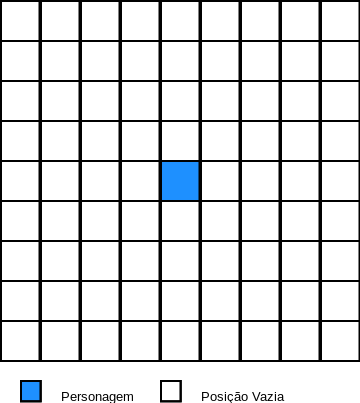
\includegraphics[height=5.0cm]{img/cap3/roi.png}
  \centering

  Fonte: O próprio autor.
\end{figure}

A partir da área de interesse do jogo, como o da Figura~\ref{fig:roi}, o robô poderá decidir suas ações baseado em um automato.
%
Caso ele alcance os extremos do mapa, ele será movimentado para outro mapa.
%
Nos casos de arquiteturas com múltiplos gerenciadores de mundo, será utilizado o comando \textit{ReBind} para realizar a conexão com o microsserviço correto após o translado do personagem.



Todas as ações do robô no mapa são baseado em um automato.
%
Nesse sentido, espera-se obter um padrão de movimentação a fim de evitar ciclos a qual um jogador comum dificilmente realizará (\textit{e.g.,} Andar para frente e para trás, ficar equipando itens em ciclo, ficar consumindo itens até acabar, \textit{etc.}).
%
A movimentação do personagem seguirá o automato descrito na Figura~\ref{fig:movimentacao}.


\begin{figure}[htb!]
  \caption{Automato de movimentação dos personagens simulados}
  \label{fig:movimentacao}
  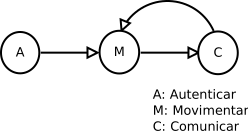
\includegraphics[height=3.5cm]{img/cap3/movimentacao.png}
  \centering

  Fonte: O próprio autor.
\end{figure}

A Figura~\ref{fig:movimentacao} descreve o comportamento de um robô no ambiente do jogo simulado.
%
Ele seguirá um padrão de procurar batalhas, batalhar, gerenciar itens do personagem e buscar novas batalhas.
%
Este conjunto de ações simula o comportamento de busca de itens dentro de um jogo \ac{mmorpg}.
%
As características específicas de cada estado é definido da seguinte forma:

\begin{itemize}
  \item Autenticar: Realizará autenticação com o serviço \textit{web} ou \textit{rpc} apropriado a arquitetura. Neste passo o robô receberá as informações do seu personagem.
  \item Buscar Inimigo: Caminhará de forma aleatória a fim de buscar um inimigo, caso não exista em sua área de interesse. Caso encontre em sua área de interesse, irá aproximar deste inimigo.
  \item Batalhar: Irá atacar um inimigo, aplicando dano a este \ac{npc}. O personagem poderá receber dano. Estes valores serão fixos baseados em seu equipamento. O personagem pode perder todos os seus pontos de vida, sendo desconectado do serviço.
  \item Gerenciar Itens: O robô irá consumir itens para recuperar pontos de vida e usar equipamentos melhores aos já utilizados.
  \item Caminhar Aleatoriamente: O personagem caminhará aleatoriamente por um número de passos máximo. Após isso, voltará a buscar uma batalha.
\end{itemize}

Espera-se com esta sequência de ações, forçar aos robôs a explorar o cenário.
%
A cada mudança de estado, o jogador irá anunciar no chat a sua troca de ação.
%
Isso contribuirá com o monitoramento do comportamento dos personagens tanto quanto usará a funcionalidade de chat.
%
Para simular a ação de resposta de um jogador, cada robô que receber uma mensagem terá uma porcentagem fixa de $25\%$ responder a sua ação no atual momento.
%
Um robô não poderá responder a ele mesmo.


Ao realizar um \textit{ReBind} ou transitar de um mapa para o outro, o estado atual do automato volta para o estado \textbf{Autenticar}.
%
Caso já esteja autenticado, continuará a sua busca por inimigos na nova região.

O ambiente final da simulação tem 3 mapas no eixo horizontal e no eixo vertical, visto que esta é a combinação mínima para que o serviço tenha um mapa central com bordas para efetuar transições de novos personagens.

%ccm Genérico/abstratpo
% Quais experimentos serão realizados, se não necessário explicitar os caso de uso e o quê espera-se de resultado.
%
% Descrever como cenários, critérios e objetivos de testes.
